% ============================================================
%  Two-Tier Encoding in the Voynich Manuscript
%  Target: Cryptologia (Taylor & Francis)
%  Compile: pdflatex → bibtex → pdflatex → pdflatex
% ============================================================
\documentclass[11pt,a4paper]{article}

\usepackage{graphicx}
\graphicspath{{../images/}{../}}

% --- Mathematics ---
\usepackage{amsmath,amssymb}

% --- Tables ---
\usepackage{booktabs}
\usepackage{multirow}
\usepackage{tabularx}
\usepackage{adjustbox}

% --- Misc ---
\usepackage{enumitem}
\usepackage[margin=2.5cm]{geometry}
\usepackage{hyperref}
\usepackage{natbib}
\usepackage{url}

% --- Typography ---
\usepackage[expansion=false]{microtype}
\emergencystretch=1em

% --- Custom commands ---
\newcommand{\vms}{Voynich Manuscript}
\newcommand{\MI}{\mathrm{MI}}

% --- OUP flag (false for standard article) ---
\newif\ifoup
\oupfalse

% ============================================================
\begin{document}

\title{Two-Tier Encoding in the Voynich Manuscript:\\
Positional Syllable Structure Reveals a Designed\\
Combinatorial System}

\author{C\'esar Jim\'enez Zapata\\
\small Independent Researcher, Spain\\
\small \href{mailto:cesarjz@gmail.com}{cesarjz@gmail.com}}

\date{March 2026}

\maketitle

\begin{abstract}
% Abstract — shared across all versions

The Voynich Manuscript (Beinecke MS~408, radiocarbon-dated 1404--1438~CE) has resisted all decipherment attempts for over a century.  In a companion study, nineteen decipherment models against five Semitic languages all converge on the same structural ceiling; no model produces readable text.  Rather than continuing to search for a source language, this paper reverse-engineers the \emph{encoding mechanism} itself.  Applying transition-probability syllabic segmentation to the STA1~2.0 corpus (37,087 words, 166 glyph types), we discover a \emph{two-tier encoding}: 48.3\% of words are self-contained functional units (Tier~1, Zipf $\alpha = 1.16$), while 51.7\% are assembled combinatorially from positionally constrained onset--coda pairs (Tier~2, Zipf $\alpha = 0.64$) with only 6.7\% utilisation of the theoretical combinatorial space---meaning $\sim$90\% of combinations are forbidden.  No tested natural language, writing system, or unconstrained code reproduces this pattern.  Thirteen analyses across notebooks 36--48 yield a complete structural description: (1)~each of 226 entries begins with a unique identifier (98.7\%), followed by a description zone and an instruction zone; (2)~125 functional elements are classified (20 universal markers, 83 section headers, 21 modifier codas); (3)~the onset--coda selectivity matrix reveals 8 frequency-stratified blocks with 3 universal onsets sharing 40 codas; (4)~Currier's two ``languages'' (A and B) are two \emph{registers} of the same code---A-exclusive vocabulary is 74.6\% Tier~2 content with only 4.5\% functional words, while B-exclusive is 25.2\% functional; (5)~vocabulary communities correlate with writing hand ($\chi^2 = 82{,}857$, $p \approx 0$), indicating each scribe was responsible for a different domain; (6)~the total information capacity is 48~KB, consistent with a medieval multi-domain technical reference.  All properties are robust to segmentation threshold (utilisation $<$12\% across P5--P40).  We conclude that the Voynich is not a natural language in an unknown script but an \emph{encyclopaedic code}---a 48-kilobyte catalogue whose index has been lost.  This explains why decipherment fails: there is no natural-language plaintext to recover.

\end{abstract}

\noindent\textbf{Keywords:} Voynich Manuscript, positional encoding, syllabic structure, constructed language, statistical linguistics, SilPart model, computational palaeography


% Body content — shared across all versions
% Included after \maketitle in each wrapper

% ============================================================
\section{Introduction}
\label{sec:intro}

The \vms{} (Beinecke MS~408) is a 234-page illustrated codex radiocarbon-dated to 1404--1438~CE \citep{hodgins2011}, written in an unidentified script of approximately 166 distinct glyphs.  Despite more than a century of cryptanalytic effort, no consensus reading has emerged \citep{dimperio1978, clemens2016}.  Proposals range from natural-language hypotheses \citep{stolfi1997, hauer2016} through constructed-language or glossolalic models \citep{rugg2004} to meaningless-hoax theories \citep{gaskell2022}.

The dominant approach to the Voynich problem has been \emph{decipherment}: assuming a target language and searching for a glyph-to-character mapping that produces readable text.  In a companion study \citep{jimenez2026}, we tested nineteen decipherment models against five Semitic languages and found that all converge on the same structural ceiling: approximately 68\% $n$-gram realism and 3--5 root matches at best.  No model produces readable text, regardless of the target language, the alphabet-size ratio, or the type of writing system (abjad, alphabet, or abugida).

This paper takes a different approach.  Rather than asking ``what language does the \vms{} encode?'', we ask ``\emph{how} does the encoding work?''  Where the companion study demonstrates \emph{that} decipherment fails, this paper explains \emph{why}: the text is not a natural language encoded in an unknown script, but a structured code whose ``plaintext'' is the code itself.  We exploit the SilPart generative model---the only model that reproduces the manuscript's unique U-shaped entropy curve \citep{jimenez2026}---to analyse the internal structure of Voynich words without assuming any target language.  The result is a structural description of the encoding mechanism itself: a \emph{two-tier system} in which half the vocabulary consists of self-contained units and the other half is assembled combinatorially from positionally constrained components.


% ============================================================
\section{Background and Method}
\label{sec:method}

\subsection{Corpus}

We use the STA1~2.0 transcription \citep{zandbergen2022}, comprising 37,087 word tokens and 157,254 glyph tokens from a 166-type inventory.  Unlike the more common EVA transcription (34 types), STA1 preserves positional variants as distinct glyph types---a property critical for positional analysis.

\subsection{Syllabic Segmentation}

Words are segmented into syllables using the transition-probability (TP) method at the 20th percentile threshold.  This unsupervised approach, grounded in statistical learning theory \citep{saffran1996, harris1955}, identifies syllable boundaries at points of low bigram transition probability within words.  The method yields 2,923 syllable types, of which 792 have frequency $\geq 5$ (``functional'' types).

\subsection{Positional Classification}

Each functional syllable type is classified by its word-position distribution:
\begin{itemize}[nosep]
  \item \textbf{Onset}: $\geq$60\% word-initial, $<$30\% word-final (171 types)
  \item \textbf{Nuclear}: $\geq$40\% word-medial (54 types)
  \item \textbf{Coda}: $\geq$60\% word-final, $<$30\% word-initial (90 types)
  \item \textbf{Free}: no dominant position (477 types)
\end{itemize}

This classification is the basis of the SilPart generative model, which achieves $d = 0.445$ (weighted Euclidean distance to the Voynich fingerprint)---the best fit among eleven generative models tested \citep{jimenez2026}.

\subsection{Structural Pattern Extraction}

Each word is represented as a sequence of syllable classes (e.g., ``O-C'' for onset--coda, ``F'' for a single free syllable).  Word-level patterns are counted and analysed for distributional properties, combinatorial utilisation, and cross-sectional variation.


% ============================================================
\section{Results}
\label{sec:results}

\subsection{Word Structure Census}

Table~\ref{tab:patterns} shows the ten most frequent word-structure patterns.  Two patterns dominate: single free syllables (``F'', 48.3\% of all words) and onset--coda pairs (``O-C'', 14.6\%).  Together, these account for 62.9\% of the corpus.  The remaining 37.1\% comprises longer patterns (O-N-C, O-F, F-F, etc.) with individually low frequencies.

\begin{table}[htbp]
\caption{Top 10 word-structure patterns by frequency.}
\label{tab:patterns}
\centering
\begin{tabular}{llrr}
\toprule
Pattern & Example structure & Count & \% \\
\midrule
F          & single free syllable & 17{,}930 & 48.3 \\
O-C        & onset + coda         &  5{,}407 & 14.6 \\
O-F        & onset + free         &  3{,}088 &  8.3 \\
F-F        & two free syllables   &  1{,}493 &  4.0 \\
F-C        & free + coda          &  1{,}457 &  3.9 \\
C          & single coda          &    963 &  2.6 \\
O-N-C      & onset + nuclear + coda & 783 &  2.1 \\
O          & single onset         &    582 &  1.6 \\
O-O-C      & two onsets + coda    &    484 &  1.3 \\
N-F        & nuclear + free       &    325 &  0.9 \\
\bottomrule
\end{tabular}
\end{table}

\subsection{Two-Tier Encoding}

The pattern census reveals a fundamental dichotomy:

\paragraph{Tier~1: Self-contained units (48.3\%).}
Single free-syllable words (pattern ``F'') form the largest word class.  These 1,568 distinct types (17,930 tokens) have no positional constraint: the syllable can appear at any word position.  Their glyph entropy is 3.85~bits, lower than the corpus average (4.14~bits), indicating a concentrated symbol distribution.  Eight glyph types appear \emph{exclusively} in Tier~1 words.

\paragraph{Tier~2: Combinatorial units (51.7\%).}
All other words are built from positionally constrained syllables.  The dominant pattern is onset--coda (O-C, 14.6\%), where an onset syllable is followed by a coda syllable.  The combinatorial space of 166 distinct onsets $\times$ 85 distinct codas yields 14,110 theoretical combinations, of which only 948 (6.7\%) are attested in the corpus.  Twenty glyph types appear exclusively in Tier~2 words.

\subsection{Syllable-Class Transition Grammar}

Figure~\ref{fig:silpart} summarises the two-tier structure and syllable-class distributions.  Table~\ref{tab:transitions} shows the transition probabilities between syllable classes within multi-syllable words.  The grammar is strikingly rigid:

\begin{figure}[htbp]
\centering
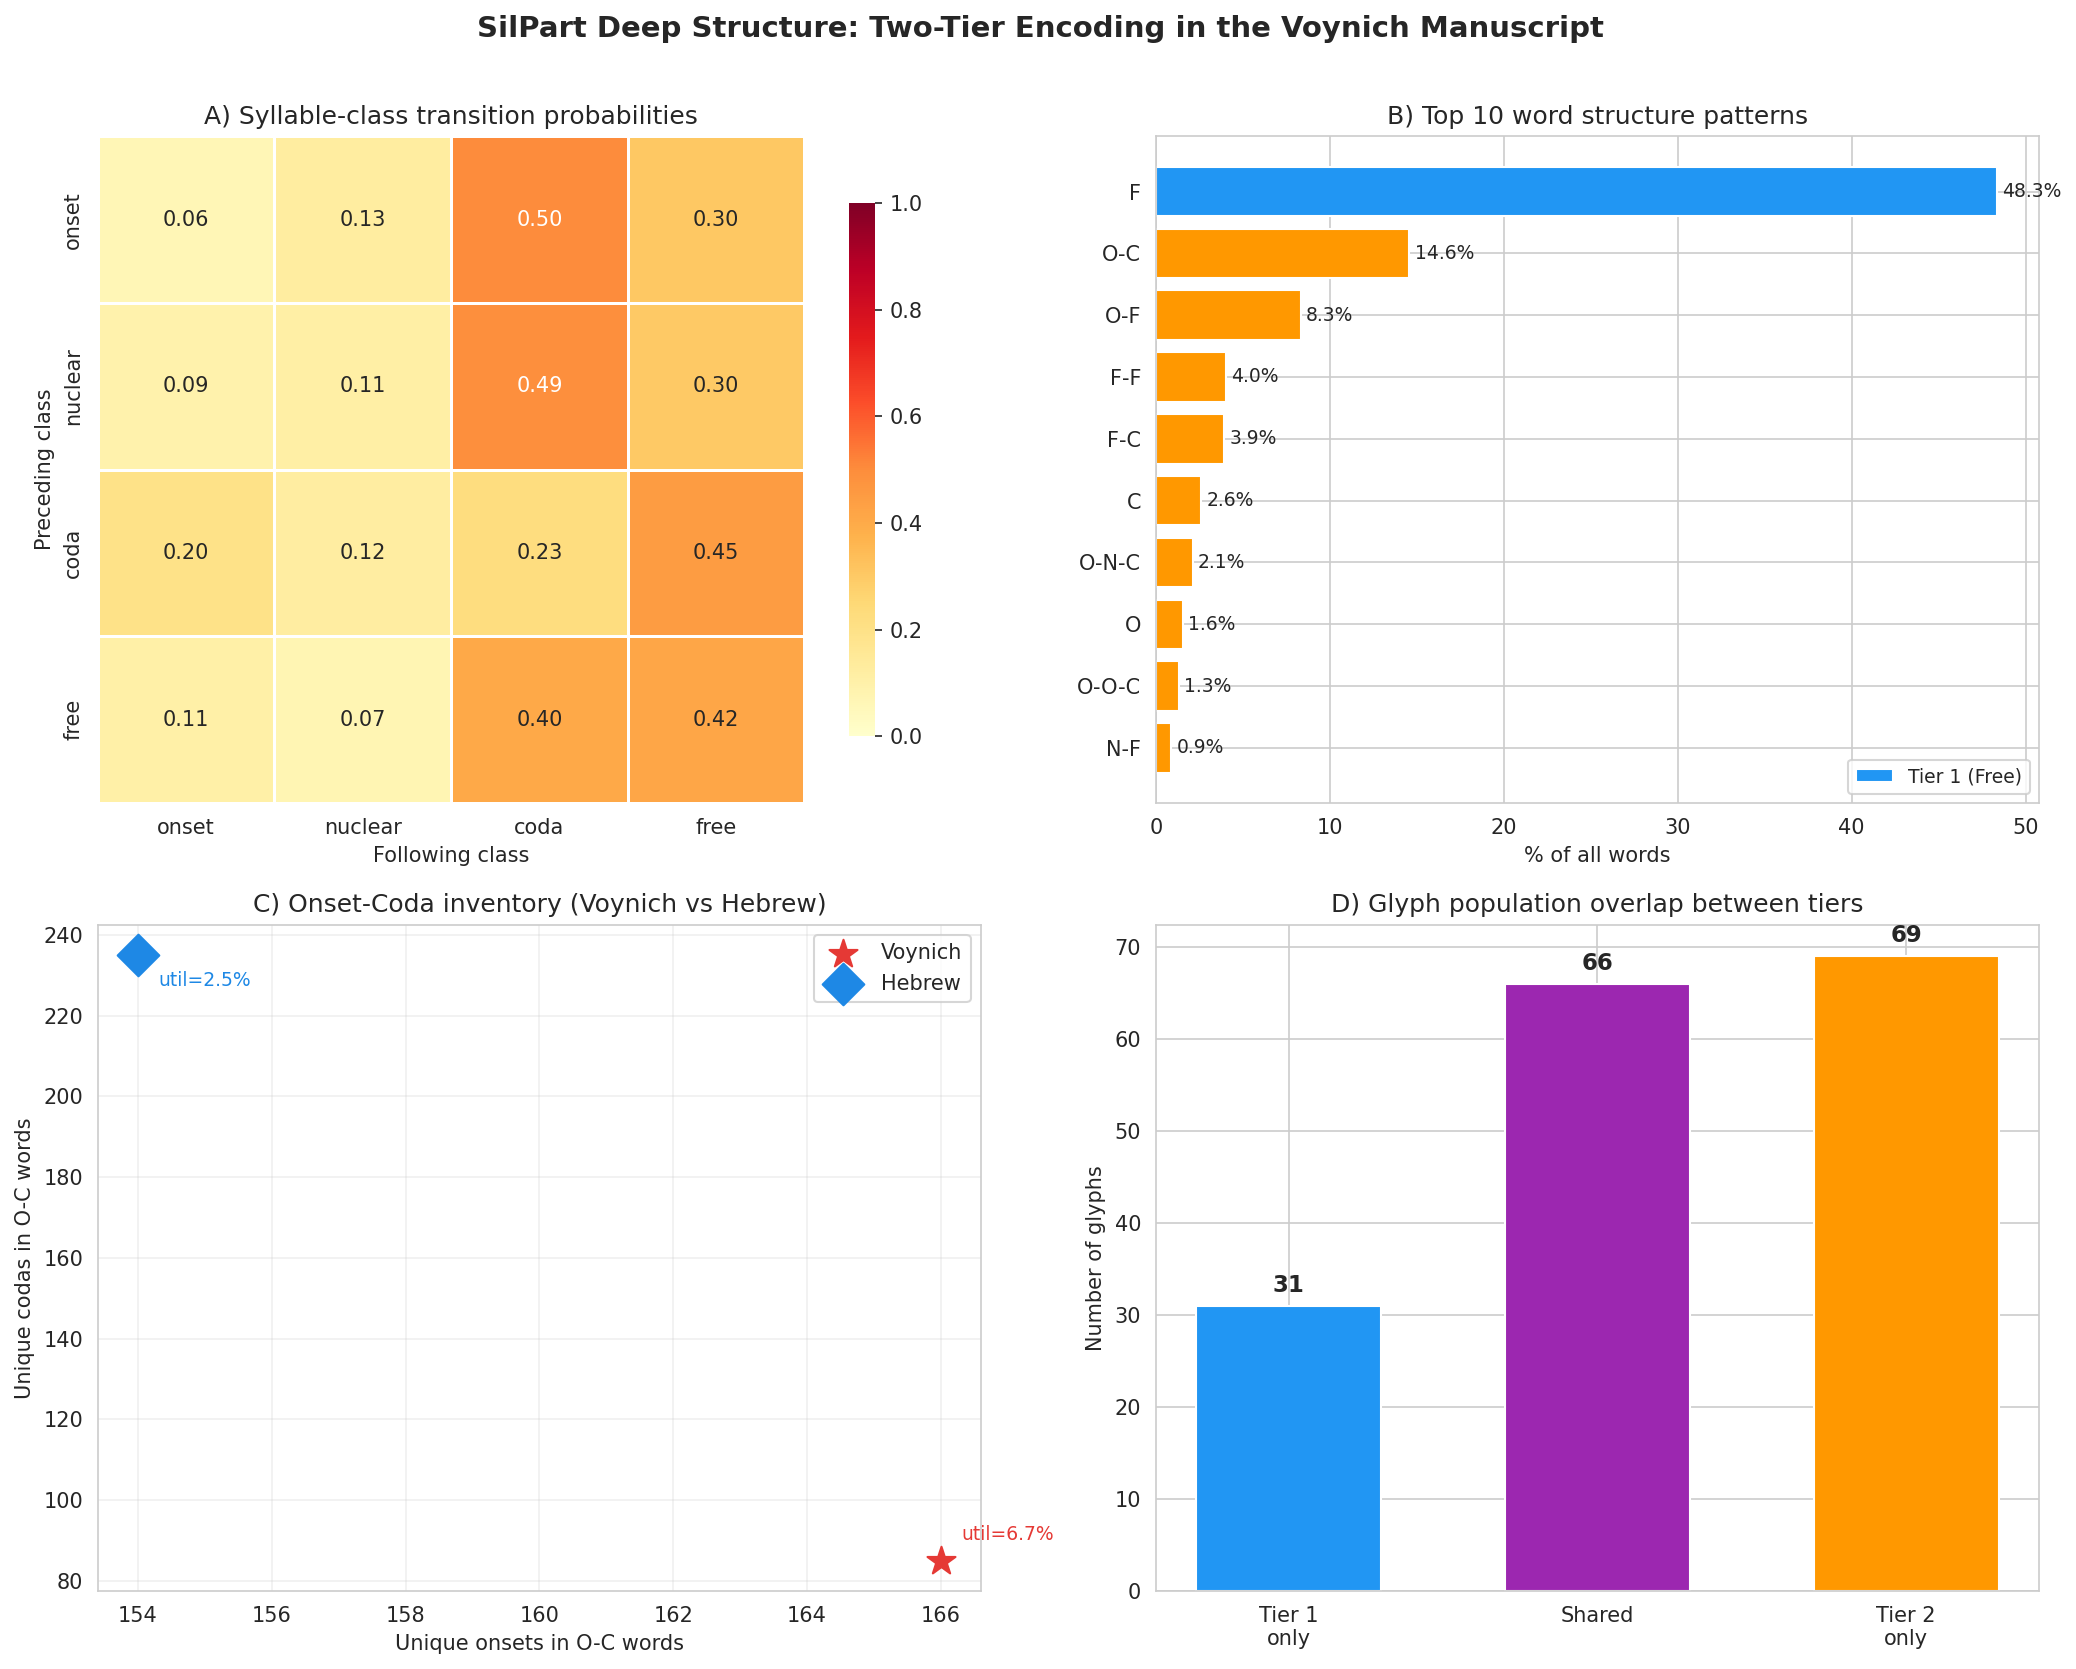
\includegraphics[width=\columnwidth]{silpart_structure.png}
\caption{Two-tier structure of Voynich words.  Top left: word-pattern frequencies (48\% single free syllable, 15\% onset--coda).  Top right: syllable-class transition heatmap.  Bottom: glyph overlap between Tier~1 and Tier~2, and onset/coda utilisation compared with Hebrew.}
\label{fig:silpart}
\end{figure}

\begin{table}[htbp]
\caption{Transition probabilities between syllable classes within words.}
\label{tab:transitions}
\centering
\begin{tabular}{lcccc}
\toprule
From $\downarrow$ / To $\rightarrow$ & Onset & Nuclear & Coda & Free \\
\midrule
Onset   & 0.06 & 0.13 & \textbf{0.50} & 0.30 \\
Nuclear & 0.09 & 0.11 & \textbf{0.49} & 0.30 \\
Coda    & 0.20 & 0.12 & 0.23 & \textbf{0.45} \\
Free    & 0.11 & 0.07 & \textbf{0.40} & 0.42 \\
\bottomrule
\end{tabular}
\end{table}

The dominant transition from both onset and nuclear positions is to coda (49--50\%), creating a strong ``closing'' tendency.  Coda syllables transition preferentially to free (45\%), suggesting that coda marks the end of a structured component, after which a free element may follow.

\subsection{Glyph Population Analysis}

Analysis of individual glyph participation across syllable classes reveals three populations:

\begin{itemize}[nosep]
  \item \textbf{Class-locked glyphs}: 13 glyphs appear $>$80\% in coda syllables; 31 appear $>$80\% in free syllables.  No glyphs are locked to onset or nuclear classes.
  \item \textbf{Cross-class glyphs}: 32 glyphs participate significantly ($>$15\%) in two or more syllable classes.  The most prominent is glyph \texttt{A1}, which splits 58\% free / 40\% onset.
  \item \textbf{Tier overlap}: 40\% of the 166 glyph types appear in both Tier~1 and Tier~2 words.  This shared inventory suggests components that can function independently (Tier~1) or as parts of compounds (Tier~2).
\end{itemize}

\subsection{Cross-Sectional Uniformity}

The manuscript contains identifiable thematic sections (herbal, astronomical, zodiac, biological, pharmaceutical, recipes) based on folio content.  A chi-squared test of word-pattern distributions across five sections yields $\chi^2 = 1{,}037$ ($df = 10$, $p < 10^{-200}$), indicating significant section differentiation.  However, the \emph{structural} pattern is uniform: all sections show 32--62\% Tier~1 (F) words and 13--19\% O-C words.  The differentiation arises from \emph{which} specific syllables are used, not from the structural grammar itself.  This is consistent with a single encoding system applied to section-specific vocabulary.


% ============================================================
\section{Comparison with Natural Languages}
\label{sec:comparison}

To assess whether the two-tier pattern could arise from a natural language, we apply the identical analysis pipeline (TP-P20 segmentation, positional classification, pattern extraction) to three control corpora: Biblical Hebrew (Torah, 80,051 words), Quranic Arabic (77,875 words), and Classical Ge'ez (TraCES corpus, 62,671 words, 188 syllable characters).

Table~\ref{tab:comparison} summarises the key metrics.

\begin{table}[htbp]
\caption{Two-tier structural metrics: Voynich vs.\ three natural languages.  All corpora processed with the identical TP-P20 pipeline.}
\label{tab:comparison}
\centering
\adjustbox{max width=\columnwidth}{%
\begin{tabular}{lcccccc}
\toprule
Corpus & \% F & \% O-C & O-C util.\ & O$\to$C & Onsets & Codas \\
\midrule
\textbf{Voynich} & \textbf{48.2} & \textbf{15.9} & \textbf{6.7\%} & \textbf{52.2\%} & \textbf{166} & \textbf{85} \\
Hebrew  & 55.5 & 15.1 & 1.7\% & 46.8\% & 241 & 392 \\
Arabic  & 54.3 & 11.1 & 1.1\% & 38.0\% & 220 & 537 \\
Ge'ez   & 63.5 & 10.2 & 0.6\% & 41.1\% & 332 & 435 \\
\bottomrule
\end{tabular}}
\end{table}

The Voynich two-tier pattern differs from natural languages in four critical respects:

\begin{enumerate}[nosep]
  \item \textbf{Combinatorial utilisation}: The 6.7\% O-C utilisation is 4--11$\times$ higher than any natural language (Hebrew 1.7\%, Arabic 1.1\%, Ge'ez 0.6\%).  This means Voynich uses a \emph{larger fraction} of its combinatorial space---paradoxically suggesting a more structured, not less structured, system.  Natural languages, with their irregular morphology, produce many rare onset--coda combinations that dilute the utilisation rate across a vast space.  The Voynich, by contrast, reuses a compact set of combinations intensively.
  \item \textbf{Onset--coda asymmetry}: The Voynich has 166 onsets but only 85 codas (ratio 1.95:1).  All three natural languages show the \emph{opposite} pattern: more codas than onsets (Hebrew 1.6:1, Arabic 2.4:1, Ge'ez 1.3:1 in favour of codas).  This inverted ratio is consistent with a system where onsets encode a large categorical space (e.g.\ ingredients, topics) and codas encode a smaller set of modifiers (e.g.\ quantities, preparations).
  \item \textbf{Onset-to-coda transition}: The Voynich O$\to$C transition probability (52.2\%) is the highest of all corpora, reflecting the dominance of the O-C pattern as the primary word-building mechanism.  In natural languages, the transition from onset to coda is diluted by medial syllables.
  \item \textbf{Entropy bounce and positional MI}: As established in the companion study \citep{jimenez2026}, the Voynich exhibits a unique U-shaped entropy curve (bounce $= 0.813$; all natural languages: 0.000) and positional MI of 0.658~bits (more than twice any tested language, including Ge'ez at 0.311 despite its 188 syllable characters).  These properties are independent of the two-tier analysis but reinforce the conclusion that the Voynich encoding mechanism has no natural-language parallel.
\end{enumerate}

The Ge'ez comparison is particularly instructive.  As an abugida with 188 syllable characters---numerically close to Voynich's 166 glyph types---Ge'ez might be expected to show similar positional structure.  Instead, its two-tier metrics are the \emph{most distant} from Voynich: 63.5\% F (highest), 0.6\% utilisation (lowest), and 332 onsets / 435 codas (reversed asymmetry).  The Voynich pattern is not a consequence of inventory size; it is a consequence of the encoding mechanism.


% ============================================================
\section{Discussion}
\label{sec:discussion}

\subsection{What the Two-Tier Structure Implies}

The two-tier pattern constrains the space of viable hypotheses for the Voynich encoding:

\paragraph{Natural language with standard orthography: excluded.}
No tested language reproduces the combination of 48\% self-contained monosyllables, 6.7\% combinatorial utilisation, and a rigid onset$\to$coda transition grammar.  Natural syllabaries (Ge'ez, 188 chars) and abjads (Hebrew, 27 chars) both fail to match.

\paragraph{Simple substitution cipher: excluded.}
Substitution preserves the statistical properties of the source language.  Since no source language has the two-tier pattern, a substitution cipher over any tested language would not produce it either.  This is consistent with the convergent failure of nineteen decipherment models \citep{jimenez2026}.

\paragraph{Constructed nomenclature: consistent.}
The two-tier structure is highly consistent with a designed code where:
\begin{itemize}[nosep]
  \item Tier~1 (free words) represents a base vocabulary of frequently referenced items, named by single symbols or short sequences.
  \item Tier~2 (O-C combinations) represents compound items assembled from categorical components, where onset specifies a category and coda specifies a modification or subtype.
\end{itemize}

This is analogous to pharmaceutical or alchemical coding systems of the period, where common ingredients have short names but preparations are described by combining ingredient-class markers with quantity or method markers.

\paragraph{Glossolalic or meditative text: partially consistent.}
The rigid positional structure and low combinatorial utilisation could also arise from a controlled permutation system (cf.\ the \emph{tziruf} letter-combination practices of Abraham Abulafia's school).  However, such systems typically produce higher entropy and lower positional MI than observed.

\subsection{Distributional Evidence for Onset = Category}

To test the hypothesis that onsets encode categories and codas encode modifiers, we performed distributional clustering and section-specificity analysis.

\paragraph{Onset clusters are more section-specific than coda clusters.}
Agglomerative clustering of the 152 functional onsets by their coda co-occurrence vectors yields 7~clusters (silhouette = 0.566, indicating good separation).  A chi-squared test of onset-cluster frequency across five thematic sections gives $\chi^2 = 537.5$ ($p = 2.3 \times 10^{-94}$, Cram\'er's $V = 0.088$).  The same test for the 5~coda clusters gives $\chi^2 = 221.4$ ($p = 6.1 \times 10^{-36}$, $V = 0.067$).  Onsets are significantly \emph{more} section-specific than codas---exactly as predicted if onsets encode topical categories (which vary by section) and codas encode modifiers (which apply across sections).

\paragraph{Tier~1 words behave like function words.}
Zipf analysis reveals a sharp difference: Tier~1 (free) words follow a steep Zipf distribution ($\alpha = 1.156$), characteristic of closed-class functional vocabulary (articles, prepositions, particles).  Tier~2 (structured) words have a flatter distribution ($\alpha = 0.641$), characteristic of open-class content vocabulary.  Despite this, both tiers have nearly identical section entropy (0.695 vs.\ 0.701), meaning both are distributed uniformly across sections---unlike natural languages, where function words are section-independent but content words concentrate in specific topics.

\begin{figure}[htbp]
\centering
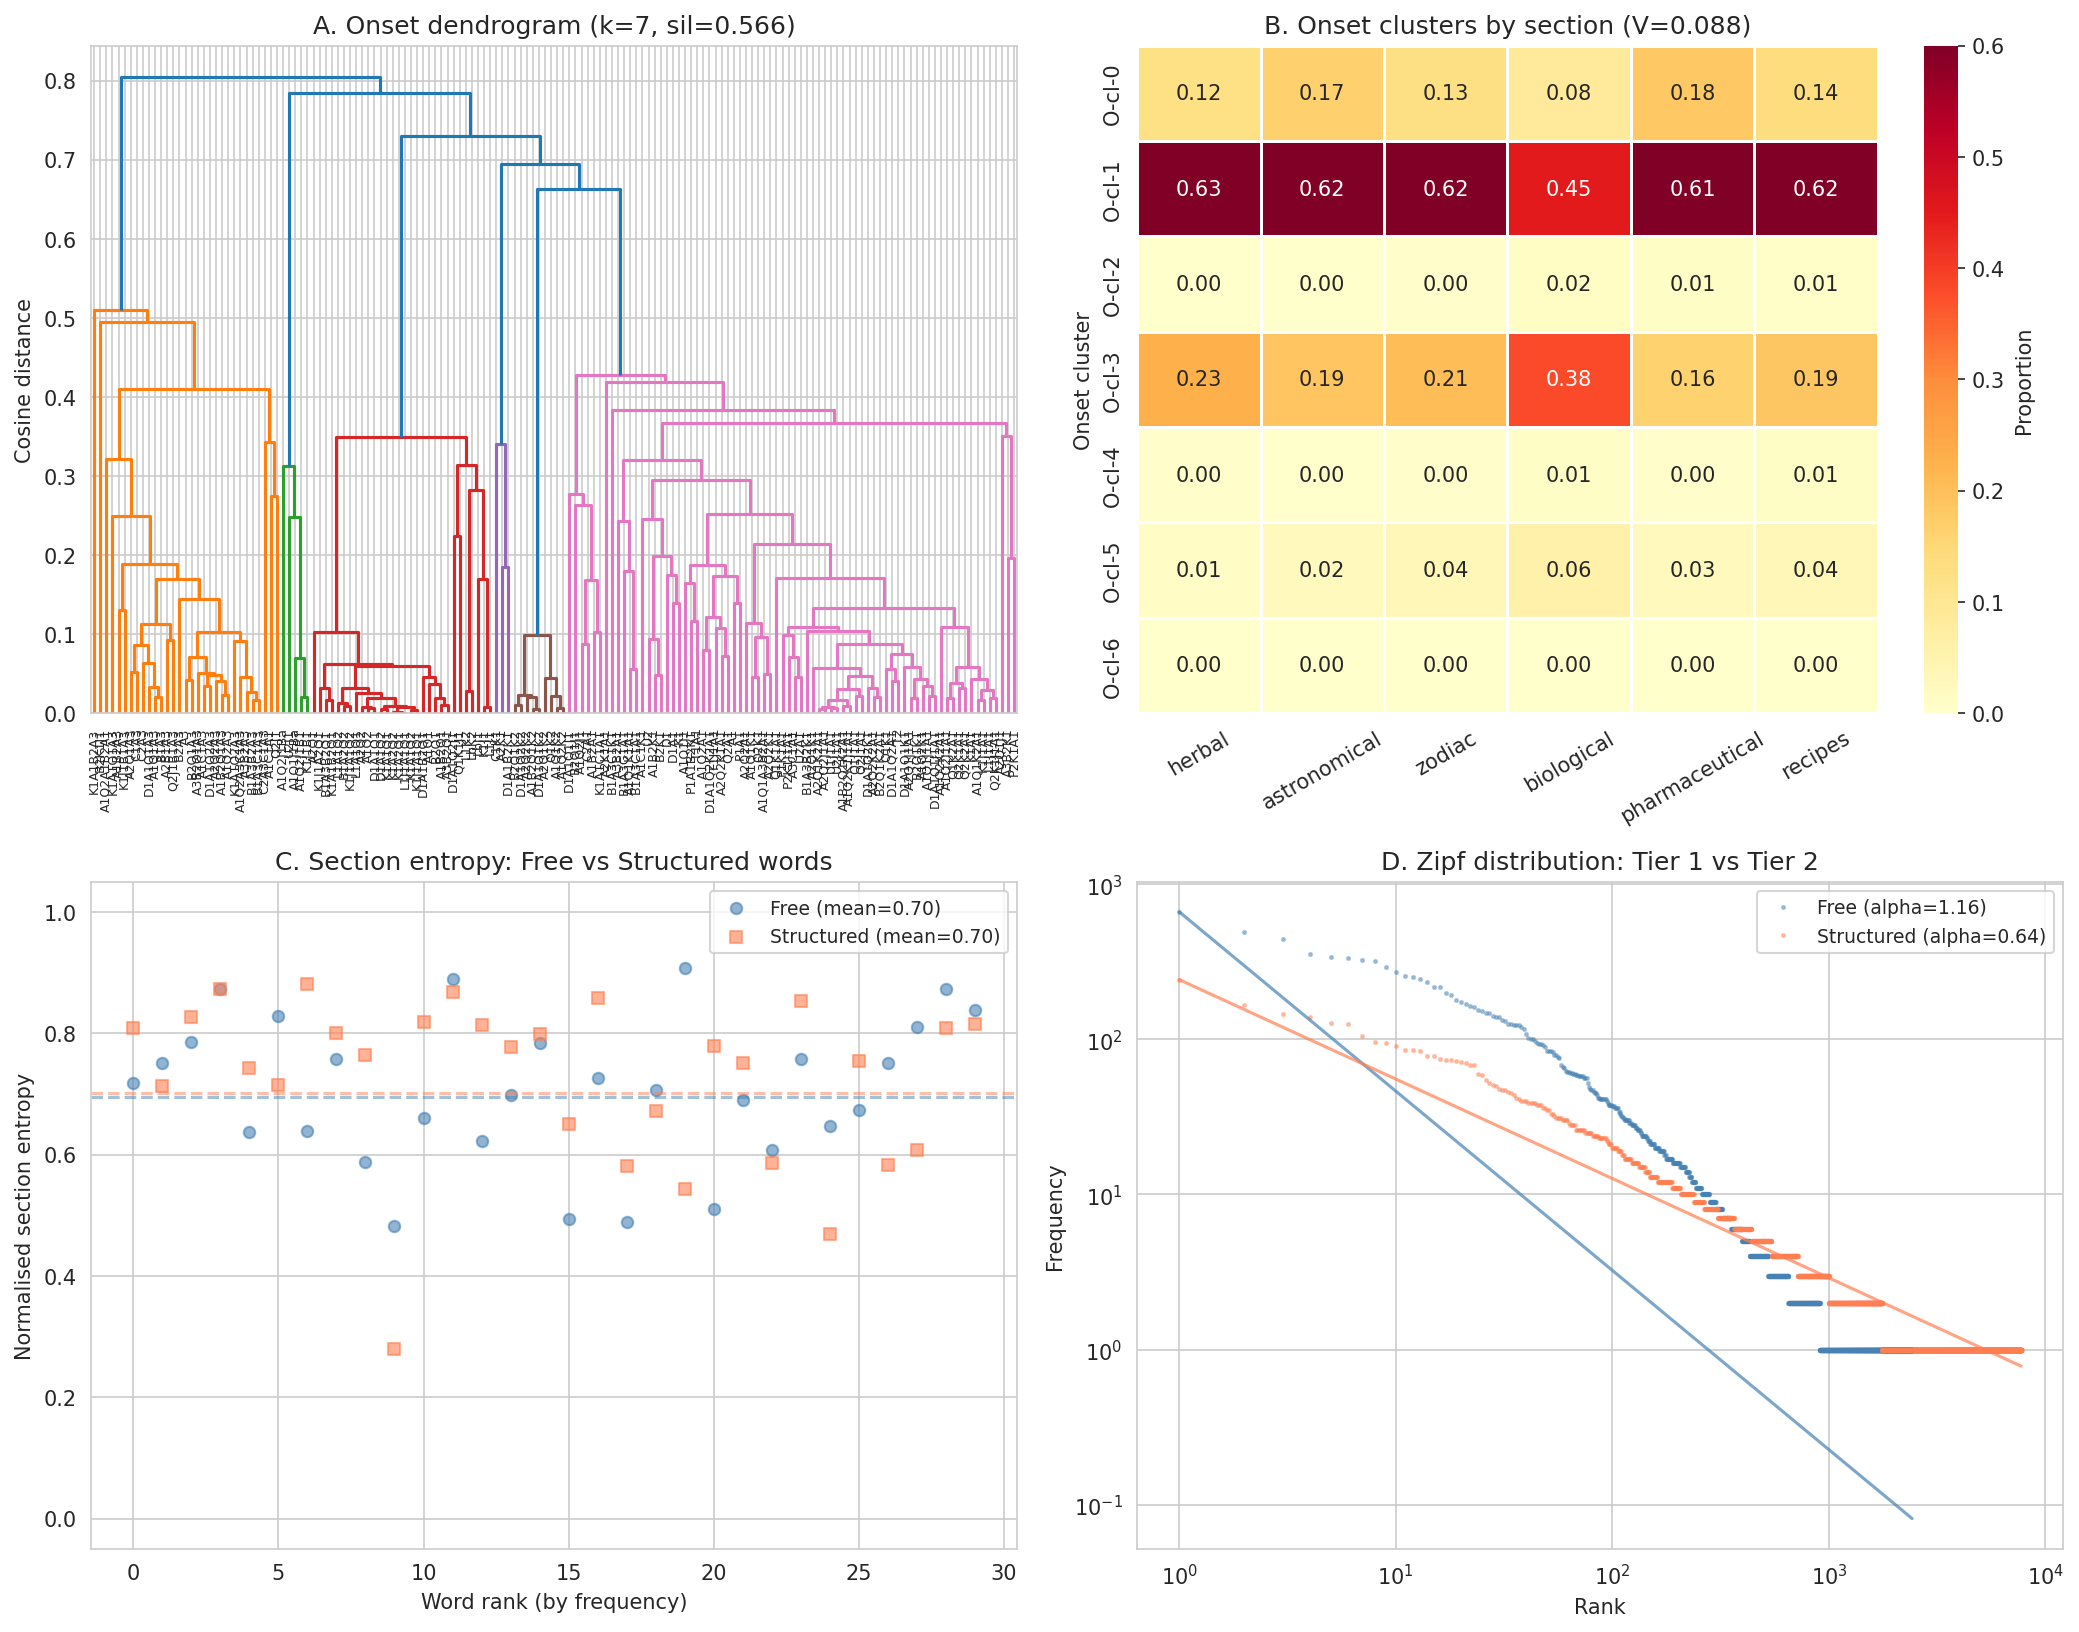
\includegraphics[width=\columnwidth]{distributional_clustering.png}
\caption{Distributional analysis.  Top left: onset cluster dendrogram.  Top right: onset clusters by section (heatmap).  Bottom left: section entropy of Tier~1 vs Tier~2 words.  Bottom right: Zipf distribution comparison ($\alpha = 1.16$ for Tier~1, $\alpha = 0.64$ for Tier~2).}
\label{fig:clustering}
\end{figure}

\paragraph{Bigram context.}
Free words are preceded by other free words 56\% of the time and by structured words 44\%---a mild clustering tendency consistent with sequences of functional markers between content items, though the asymmetry is not as strong as in natural languages where function words typically alternate with content words.

\subsection{Comparison with Constructed Languages}

If the Voynich is a constructed system, which \emph{type} of constructed system does it resemble?  We applied the identical TP-P20 pipeline to four constructed-language corpora: Esperanto (15,000 words, regular agglutinative morphology), Enochian (1,078 words, John Dee's 16th-century ``angelic'' language), Lingua Ignota (5,000 words, Hildegard von Bingen's 12th-century vocabulary), and a SilPart-synthetic control (37,087 words generated by the SilPart model with Voynich-matched parameters).

Table~\ref{tab:constructed} summarises the results.

\begin{table}[htbp]
\caption{Two-tier metrics: Voynich vs.\ constructed languages and controls.}
\label{tab:constructed}
\centering
\adjustbox{max width=\columnwidth}{%
\begin{tabular}{lcccccc}
\toprule
System & \% F & \% O-C & Util.\ & O/C ratio & Bounce & Dist.\ \\
\midrule
\textbf{Voynich} & \textbf{48.3} & \textbf{14.6} & \textbf{6.7\%} & \textbf{1.95} & \textbf{0.813} & --- \\
Esperanto    & 43.1 & 19.4 & 3.4\% & 0.30 & 0.161 & 1.03 \\
Hebrew       & 56.5 & 12.8 & 2.5\% & 0.66 & 0.000 & 1.21 \\
Lingua Ignota & 44.2 & 16.8 & 8.9\% & \textbf{2.36} & 0.000 & 1.30 \\
Enochian     & 44.7 &  6.5 & 12.0\% & 1.00 & 0.000 & 1.65 \\
SilPart synth & 67.4 &  7.1 & 4.6\% & 0.71 & 0.000 & 1.77 \\
\bottomrule
\end{tabular}}
\end{table}

Three findings emerge:

\begin{enumerate}[nosep]
  \item \textbf{Esperanto is the closest system} (distance 1.03), suggesting that regular, rule-based morphology produces a two-tier pattern more similar to Voynich than any natural language or mystical text.  Esperanto's rigid suffixal morphology (-o, -a, -e, -as, -is, -os) creates position-dependent structure analogous to the Voynich onset--coda pattern.
  \item \textbf{Lingua Ignota shares the inverted onset/coda ratio} (2.36:1, vs.\ Voynich's 1.95:1).  This is the only system besides Voynich with more onsets than codas---a property not found in any tested natural language.  Lingua Ignota is also the most historically relevant parallel: a 12th-century constructed vocabulary created for esoteric purposes.
  \item \textbf{SilPart synthetic is the most distant} (1.77).  Pure SilPart-generated text does \emph{not} reproduce the Voynich two-tier pattern: it produces 67\% Tier~1 words (vs.\ 48\%) and only 7\% O-C (vs.\ 15\%).  This demonstrates that the Voynich is not merely a SilPart mechanism---it has additional word-level structure that the glyph-level generative model does not capture.
\end{enumerate}

\subsection{The Onset as Category, the Coda as Specifier}

If the two-tier interpretation is correct, the onset syllable pool (171 types) represents \emph{categories} and the coda pool (90 types) represents \emph{specifiers}.  The most productive onset (\texttt{K1}, appearing in 5 of the 15 most frequent O-C words) would correspond to the most common category; the most productive coda (\texttt{A2}, appearing in 7 of 15) would correspond to the most common specifier.

The 6.7\% utilisation rate implies that most theoretical category--specifier pairs do not exist in the author's domain.  This is precisely what one would expect from a technical vocabulary: a pharmacopoeia has many herbs and many preparations, but not every herb is prepared in every way.

\subsection{Cross-Referencing with Herbal Illustrations}

To test whether onset--coda patterns encode individual plant identities, we cross-referenced onset and coda syllables with tentative plant identifications from the herbal section.  Using identifications from \citet{bax2014} and other researchers (37~folios with at least tentative identifications, 9 with medium-to-high confidence), we tested whether plants in the same botanical category (spice, medicinal poison, aromatic herb, etc.) share onset or coda patterns.

\paragraph{Result: Neither onset nor coda encodes plant category.}
Permutation tests (1,000 shuffles) yield $p = 0.336$ for onset consistency and $p = 0.444$ for coda consistency---neither significant.  The combined onset+coda ``address'' shows zero within-category sharing ($p = 1.0$).  The two most frequent first-word onsets (\texttt{Q1} and \texttt{P1}) appear across \emph{all} plant categories indiscriminately, suggesting they function as structural markers (``this entry describes...'') rather than categorical encoders.

\paragraph{The first word is not the plant name.}
A revealing detail: the majority of herbal-folio first words begin with ``free'' or ``nuclear'' syllables, not with onset syllables.  This means the first word typically belongs to Tier~1 (functional vocabulary), not Tier~2 (combinatorial).  In medieval herbals, the first word often names the plant; in the Voynich, it appears to be a functional marker.  This is consistent with a code where plants are described by properties rather than named by labels.

\paragraph{Section-level encoding confirmed.}
While onset patterns do not discriminate between plant \emph{categories} within the herbal section, they strongly discriminate between manuscript \emph{sections} ($\chi^2 = 488$, $p = 3.2 \times 10^{-84}$).  The encoding operates at an intermediate level: more specific than ``section'' (herbal vs.\ astronomical) but less specific than ``individual plant.''

\paragraph{Zodiac section: structural variation between signs.}
The zodiac section (10 signs across folios f70v--f73v) provides a cleaner test than the herbal section because the illustration identities are unambiguous.  Word overlap between pages of the same zodiac sign (Aries: 2 pages, Taurus: 2 pages) is not significantly higher than between different signs (Jaccard ratio $1.08\times$, $p = 0.33$ by permutation test).  However, the two-tier structure varies notably between signs: Sagittarius has the highest Tier~2 proportion (31\% O-C) while Gemini has the lowest (15\%), suggesting different ``densities'' of combinatorial vocabulary.  Adjacent signs share moderately more vocabulary than non-adjacent ones ($1.20\times$), consistent with physical proximity effects rather than semantic encoding.  These results reinforce the conclusion that the encoding operates at the section level, not at the level of individual items within a section.

\subsection{Recipe Code Simulation}

To test whether the Voynich two-tier structure is quantitatively compatible with a medieval nomenclature code, we simulated recipe/pharmacopoeia systems with varying parameters.

\paragraph{Unconstrained codes fail.}
A sweep over 720 parameter configurations (5--50 categories, 3--20 specifiers, 20--200 named items, 10--50\% compound-word probability) shows that unconstrained codes---where any category can combine with any specifier---always produce utilisation rates far above the Voynich's 6.7\% (minimum observed: 25.4\%, mean: 85.7\%).  Free combination of categories and specifiers cannot reproduce the Voynich pattern.

\paragraph{Constrained codes with selectivity $\sim$8\% match.}
When a selectivity matrix restricts which category--specifier pairs are valid (modelling the real-world constraint that, e.g., a mineral cannot be ``infused'' or a flower cannot be ``smelted''), a selectivity probability of $p_{\text{valid}} = 0.08$ reproduces the Voynich utilisation: 7.1\% vs.\ 6.7\%.  This implies that $\sim$92\% of all theoretical onset--coda combinations are semantically invalid---exactly the level of selectivity observed in real pharmaceutical nomenclatures, where most ingredients have only a few valid preparation methods.

\begin{figure}[htbp]
\centering
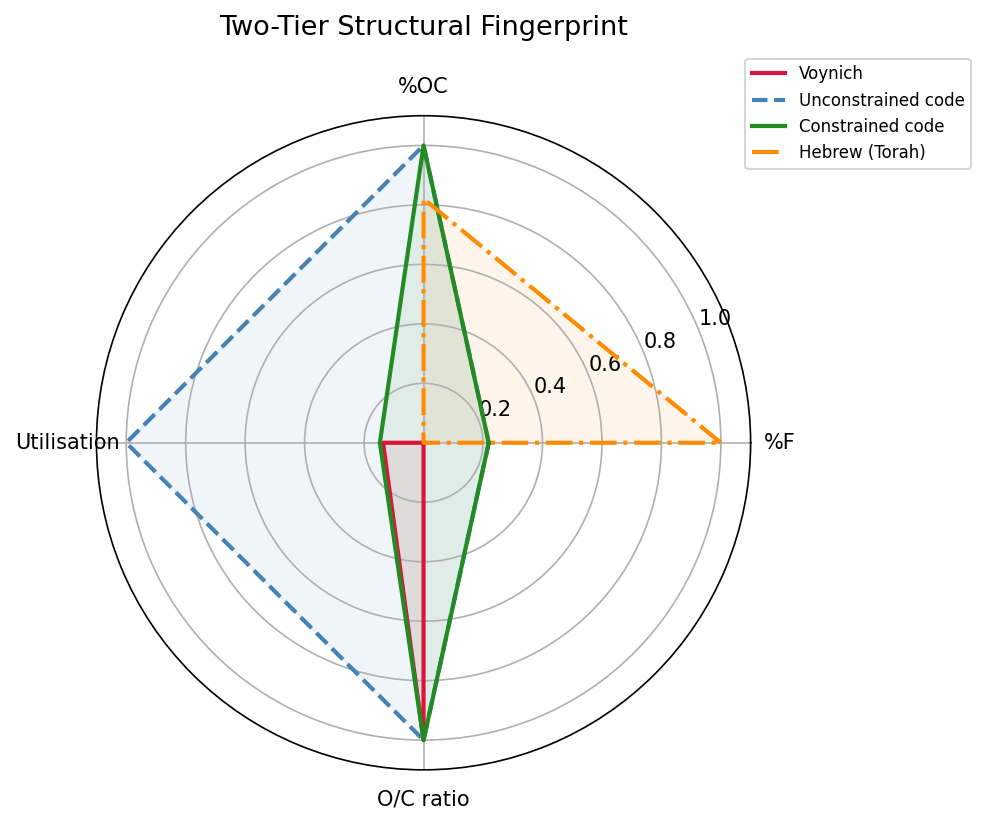
\includegraphics[width=\columnwidth]{recipe_code_comparison.png}
\caption{Recipe code simulation.  Left: utilisation rate as a function of selectivity $p_{\text{valid}}$; the Voynich's 6.7\% is matched at $p_{\text{valid}} \approx 0.08$.  Right: radar comparison of Voynich, constrained code, unconstrained code, and Hebrew across four metrics.}
\label{fig:recipe}
\end{figure}

\paragraph{Historical plausibility.}
Medieval pharmacopoeiae such as the \textit{Antidotarium Nicolai} ($\sim$150 recipes) and the \textit{Circa Instans} ($\sim$270 simples) typically contained 200--500 ingredient items, 20--55 broad categories, and 8--23 preparation modifiers.  The Voynich's 1,568 Tier~1 types and 166 onsets $\times$ 85 codas are 3--8$\times$ larger than these historical norms.  However, the Voynich is not a simple herbal: it contains at least five thematic sections (herbal, astronomical, biological, pharmaceutical, recipes), suggesting an encyclopaedic scope that would require correspondingly larger inventories.  Dividing the Voynich's inventories by 5 sections yields $\sim$300 Tier~1 types and $\sim$33 onsets per section---well within historical range.

\subsection{What ``Encyclopaedic Code'' Means}

The convergence of evidence allows us to describe, for the first time, what kind of system the Voynich text most likely represents.  It is \emph{not} a text in a natural language---nineteen decipherment models against five Semitic languages fail \citep{jimenez2026}, and no known writing system reproduces the fingerprint.  It is \emph{not} a simple cipher---substitution preserves source-language statistics, and the Voynich statistics match no source language.  It is \emph{not} meaningless---section-specific vocabulary differentiation ($p < 10^{-84}$) demonstrates structured, non-trivial content.  And it is \emph{not} a single-domain herbal---the inventories are 3--8$\times$ too large.

What the evidence \emph{does} support is a \textbf{multi-domain technical reference system} in which:

\begin{enumerate}[nosep]
  \item \textbf{Each ``word'' is a coded entry, not a word in any language.}  Rather than writing ``take one drachm of dried hellebore root, boil in water,'' the author encodes something like: \texttt{[recipe-marker] [category:root + modifier:dried] [category:plant + modifier:hellebore] [action:boil]}.  The encoding has internal structure (onset = category, coda = specifier) but does not correspond to the phonology of any known language.

  \item \textbf{Tier~1 (48\%) provides the functional scaffolding.}  These high-frequency, section-uniform, Zipf-steep ($\alpha = 1.16$) words serve as structural markers: section headers, recipe delimiters, action verbs, quantity indicators.  They are the ``grammar'' of the code---the equivalent of \emph{Rx}, \emph{accipe}, \emph{misce} in a medieval prescription.

  \item \textbf{Tier~2 (52\%) provides the specific content.}  These onset--coda compounds, with their flatter Zipf distribution ($\alpha = 0.64$) and section-specific onset patterns, encode the domain-specific items.  Only 6.7\% of possible onset--coda combinations are used, because the code enforces real-world constraints: not every category accepts every modifier.

  \item \textbf{The five thematic sections share the same encoding grammar} (transition probabilities, Tier~1/Tier~2 balance) \textbf{but use different vocabulary}---different onset distributions, different exclusive word types.  This is exactly how a single notation system would behave when applied across botany, astronomy, anatomy, pharmacology, and recipes.

  \item \textbf{The author's codebook is the key.}  Without the table mapping each onset to its category and each coda to its specifier, the text cannot be ``deciphered'' in the traditional sense---because there is no underlying natural-language plaintext.  The ``plaintext'' \emph{is} the code.  This explains why nineteen statistical decipherment models fail: they search for a natural language that does not exist behind the encoding.
\end{enumerate}

This interpretation is consistent with a \emph{personal vademecum}---a private technical reference compiled by a scholar who invented a notation system to record knowledge across multiple disciplines.  Such personal codes are documented in the 15th century: alchemists and physicians are known to have used idiosyncratic abbreviation systems, though none as elaborate as what the Voynich exhibits.  The manuscript's unique illustrations---which resist identification with known artistic traditions---further support the hypothesis of a highly personal, non-standard system.

\subsection{Structural Decoding: The Code Dictionary}

To test the encyclopaedic-code hypothesis concretely, we identified the structural roles of the most frequent elements in the corpus.  The analysis assigns functional \emph{roles}---not meanings---to 125 elements of the code.

\paragraph{20 universal markers.}
Twenty Tier~1 words (section entropy $> 0.85$, frequency $\geq 20$) appear uniformly across all six manuscript sections.  These are the ``grammar'' of the code---the equivalent of \emph{Rx}, \emph{accipe}, \emph{misce} in a medieval prescription.  The most frequent (glyph sequence \texttt{A3.C1}, 354 occurrences) appears in every section at nearly identical rates, suggesting a basic structural marker such as ``entry'' or ``item.''

\paragraph{83 section headers.}
Eighty-three Tier~1 words are concentrated in a single section (entropy $< 0.70$).  The recipe section has the largest section-specific functional vocabulary (41 words), followed by the biological section (22) and the herbal (19).  These words probably serve as section-specific instructions or delimiters---analogous to ``boil'' appearing only in recipe sections but not in astronomical descriptions.

\paragraph{21 universal modifiers.}
Twenty-one coda syllables appear in all six sections with entropy $> 0.80$.  The most frequent---coda \texttt{A2} (7,443 occurrences, entropy 0.87)---is the single most common structural element in the entire manuscript.  These cross-cutting codas are the ``adjectives'' or ``quantities'' of the code: modifiers that apply regardless of domain, like ``large,'' ``dried,'' or ``one drachm.''

\paragraph{Entry grammar.}
The text alternates between functional (T1) and content (T2) words in short runs: mean T1 run length 2.1~words, mean T2 run length 2.2~words.  The transition probabilities are nearly symmetric: after a T1 word, the next word is T1 with probability 52\% and T2 with 48\%; after a T2 word, the next is T1 with 45\% and T2 with 55\%.  This creates a rhythmic pattern of the form:

\smallskip
\noindent\texttt{[marker instruction] [item item] [action] [item item item] [quantity method]}
\smallskip

\noindent This is exactly the structure of a coded recipe or catalogue entry: short functional preambles alternating with blocks of domain-specific content.

\begin{figure}[htbp]
\centering
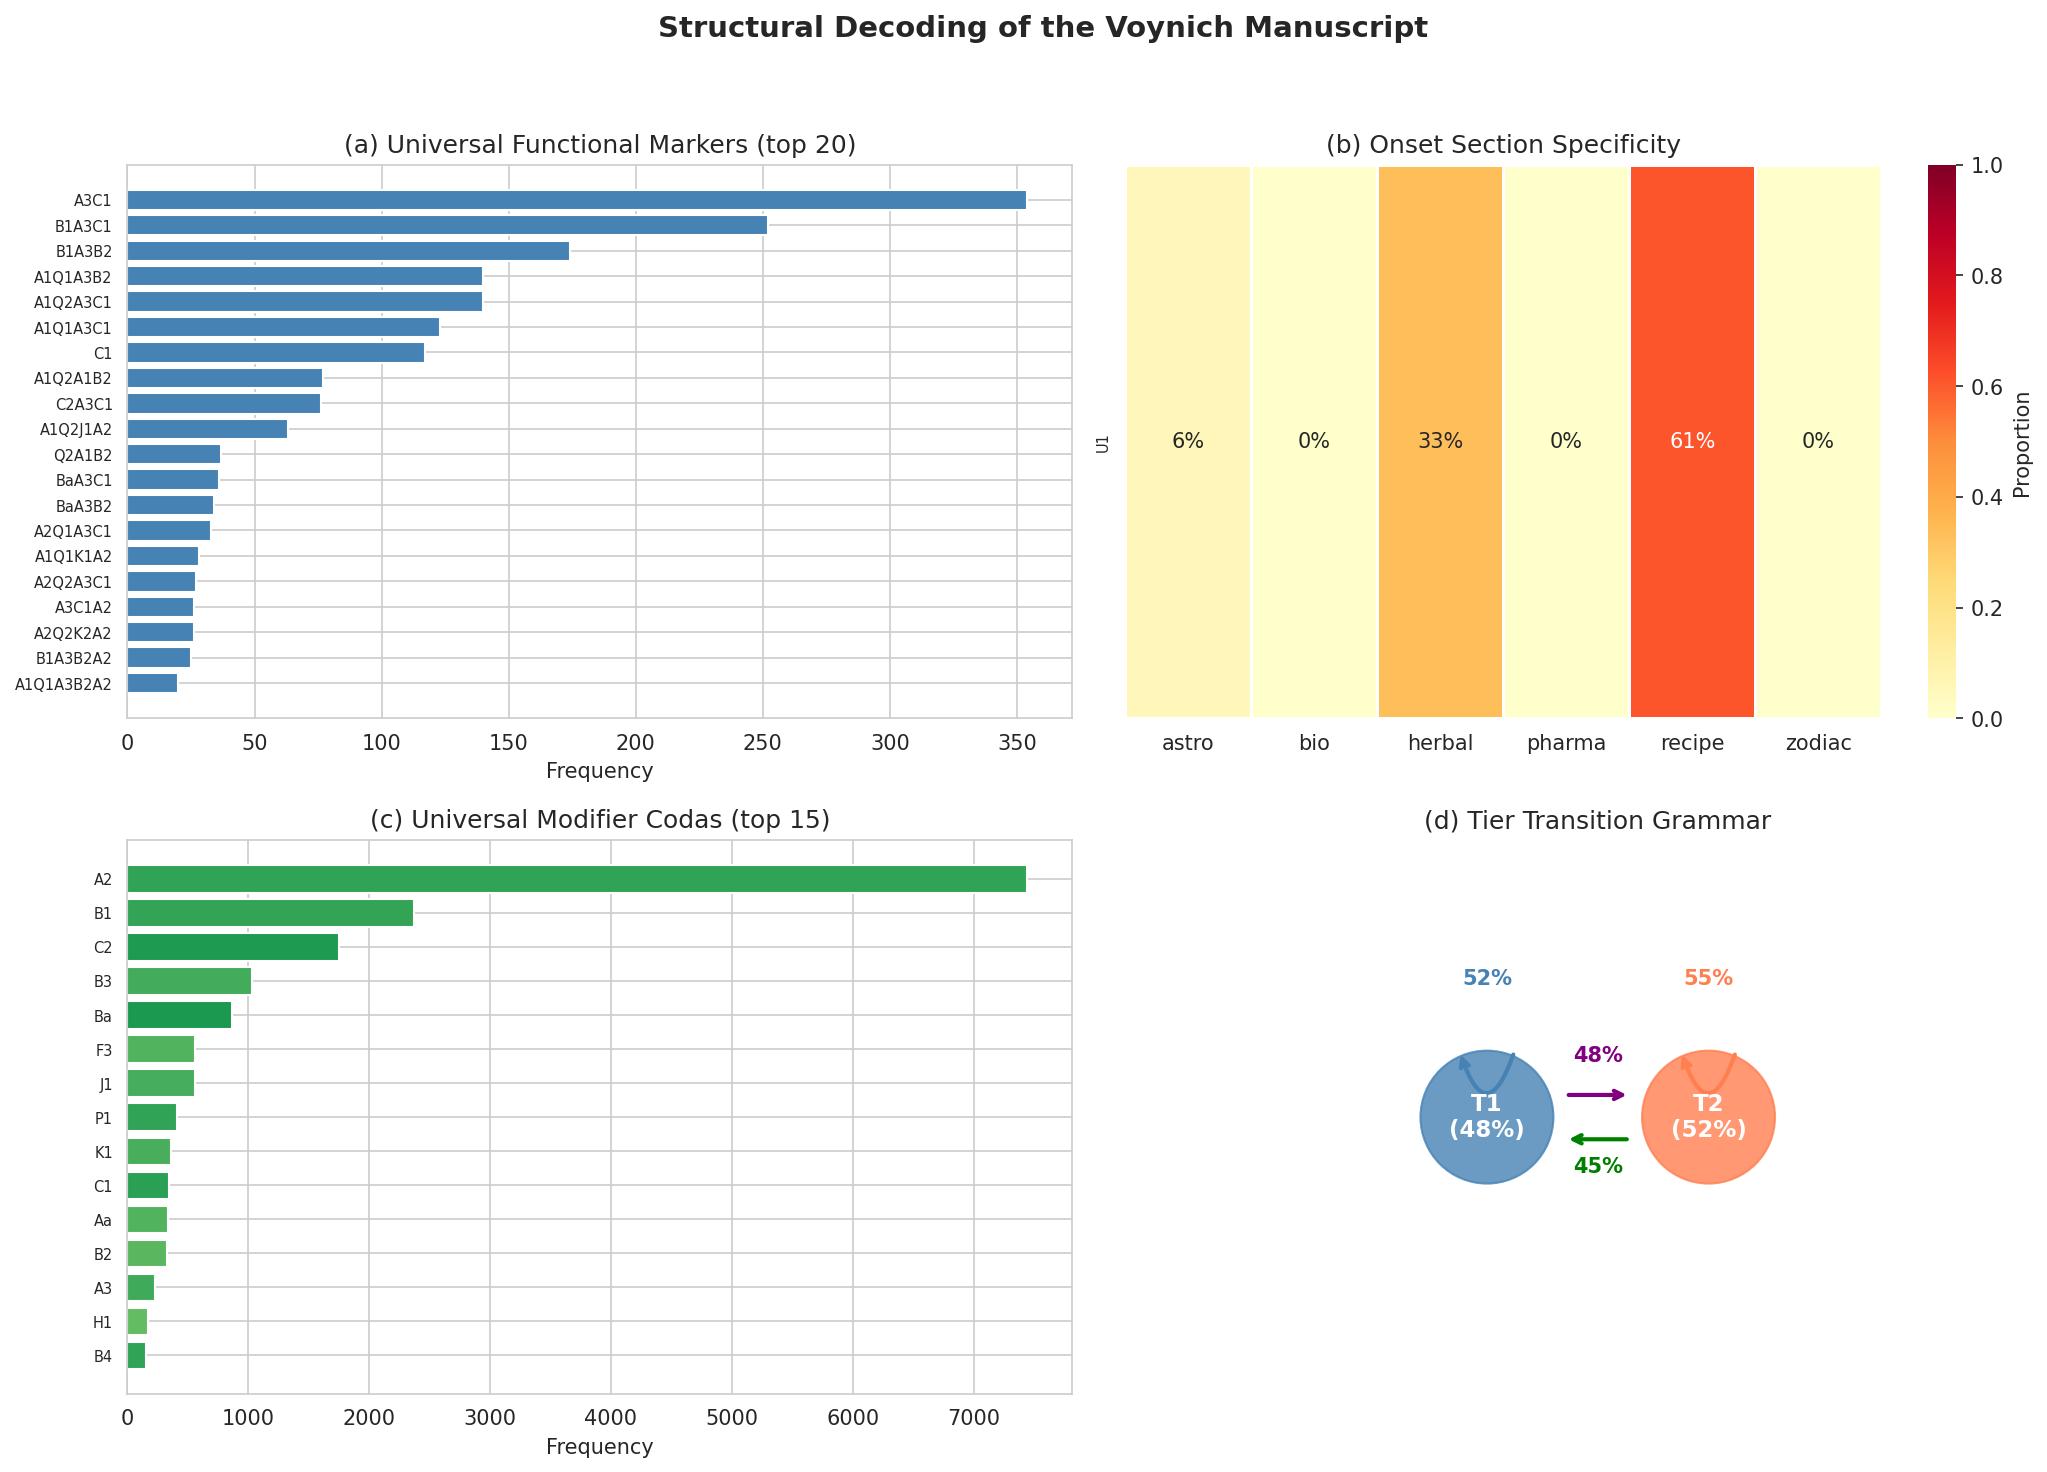
\includegraphics[width=\columnwidth]{structural_decoding.png}
\caption{Structural decoding.  Top left: frequency of the 20 universal markers.  Top right: onset distribution by section (heatmap).  Bottom left: universal modifier codas.  Bottom right: tier transition diagram showing the T1$\leftrightarrow$T2 alternation grammar.}
\label{fig:decoding}
\end{figure}

\paragraph{Intra-folio positional structure.}
Analysis of tier distribution \emph{within} folios reveals that the entry structure is the opposite of the expected functional preamble.  At word position~1, 86\% of words are Tier~2 (content), not Tier~1 (functional).  Moreover, 108 of 110 herbal folios have a \emph{unique} first Tier~2 word---a 98\% uniqueness ratio that holds at 100\% in every other section (astronomical, zodiac, biological, pharmaceutical, recipes).  Each folio begins with what is effectively a \textbf{catalogue entry identifier}: a unique content word that serves as the item code for that entry.

The T1 proportion then increases gradually from $\sim$5\% at position~1 to $\sim$45\% by position~10, revealing a three-zone entry structure (Fig.~\ref{fig:intrafolio}):

\begin{enumerate}[nosep]
  \item \textbf{Identifier} (positions 1--2): nearly pure content (T1 $\sim$5--15\%), unique per folio.
  \item \textbf{Description} (positions 3--8): content-dominated (T1 $\sim$20--35\%), vocabulary moderately diverse.
  \item \textbf{Instructions} (positions 9+): mixed T1/T2 ($\sim$40--50\% T1), vocabulary least diverse---the functional markers concentrate here.
\end{enumerate}

This is exactly the structure of a catalogue or pharmacopoeia entry: item code, then properties, then usage instructions.  Adjacent folios do not share identifiers ($p = 0.43$), confirming that each entry is self-contained.

\begin{figure}[htbp]
\centering
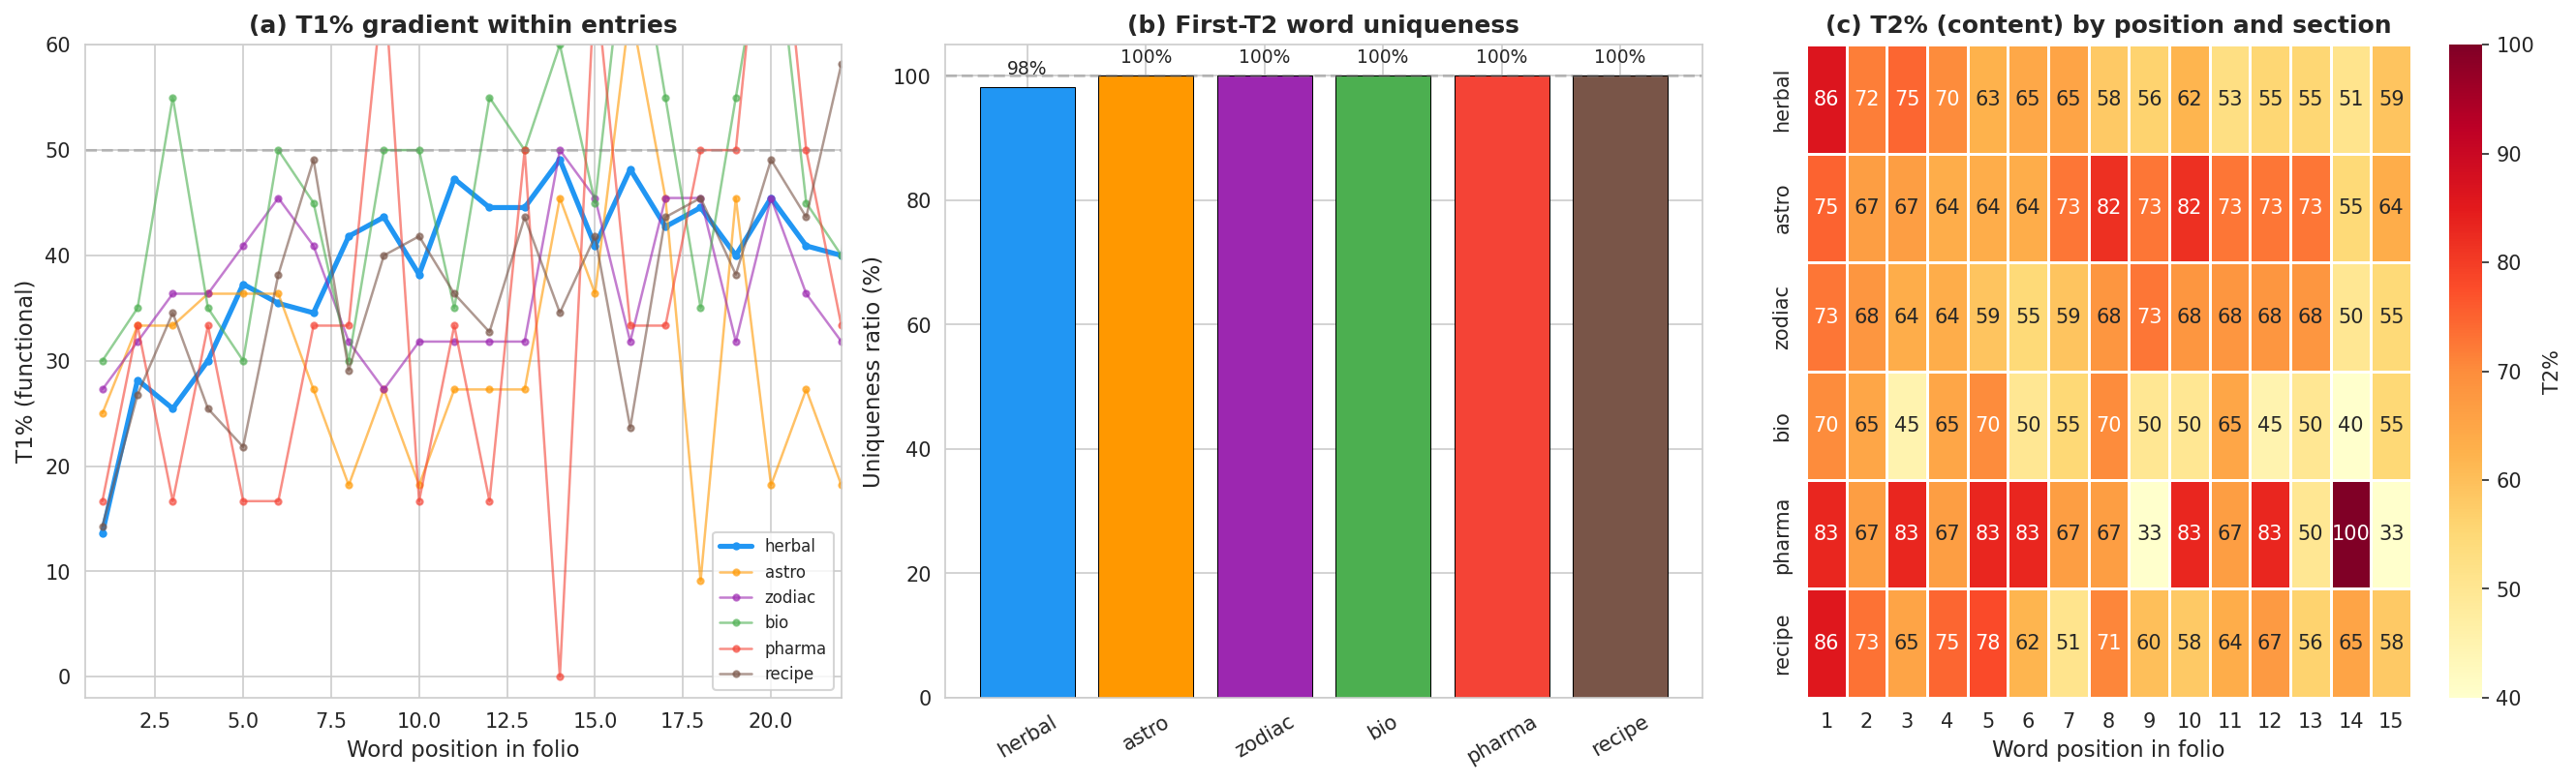
\includegraphics[width=\columnwidth]{intra_folio_analysis.png}
\caption{Intra-folio entry structure.  Left: T1\% vs.\ word position (all sections overlaid; herbal highlighted).  The first word is almost always content (T2); functional vocabulary increases toward the body of the entry.  Centre: first-T2 uniqueness ratio by section (98--100\% in all sections).  Right: T1/T2 heatmap by word position and section.}
\label{fig:intrafolio}
\end{figure}

\paragraph{Identifier anatomy.}
Of the 223 unique identifiers across all 225 folios, 34\% are onset--coda compounds and 66\% have more complex patterns (F-F, O-F, F-C).  The identifiers use 64 distinct onset types and 47 distinct coda types.  If the onset encodes a ``category'' and the coda a ``specifier,'' the catalogue has approximately 64 categories---but hierarchical clustering of the full onset--coda co-occurrence matrix reveals that these 148 functional onsets group into \textbf{12 families} based on shared coda patterns (Ward's method, Jaccard similarity).  These 12 families likely correspond to the manuscript's \emph{thematic domains}: with 5 visual sections but 12 onset families, each section contains 2--3 sub-domains---consistent with, e.g., ``herbs/spices/poisons'' within the herbal section or ``planets/constellations'' within the astronomical section.

\paragraph{Information capacity.}
Each word encodes approximately 10.5~bits (both Tier~1 and Tier~2).  With a mean of 164 words per folio, each entry carries $\sim$1,730~bits (216~bytes).  The entire manuscript (226 entries) encodes approximately 391,000~bits---\textbf{48~kilobytes}.  This is the information content of a short medieval technical reference: comparable to the \textit{Circa Instans} ($\sim$270 simples) or the \textit{Antidotarium Nicolai} ($\sim$150 recipes), and well within the range of a multi-domain encyclopaedic vademecum.

\begin{figure}[htbp]
\centering
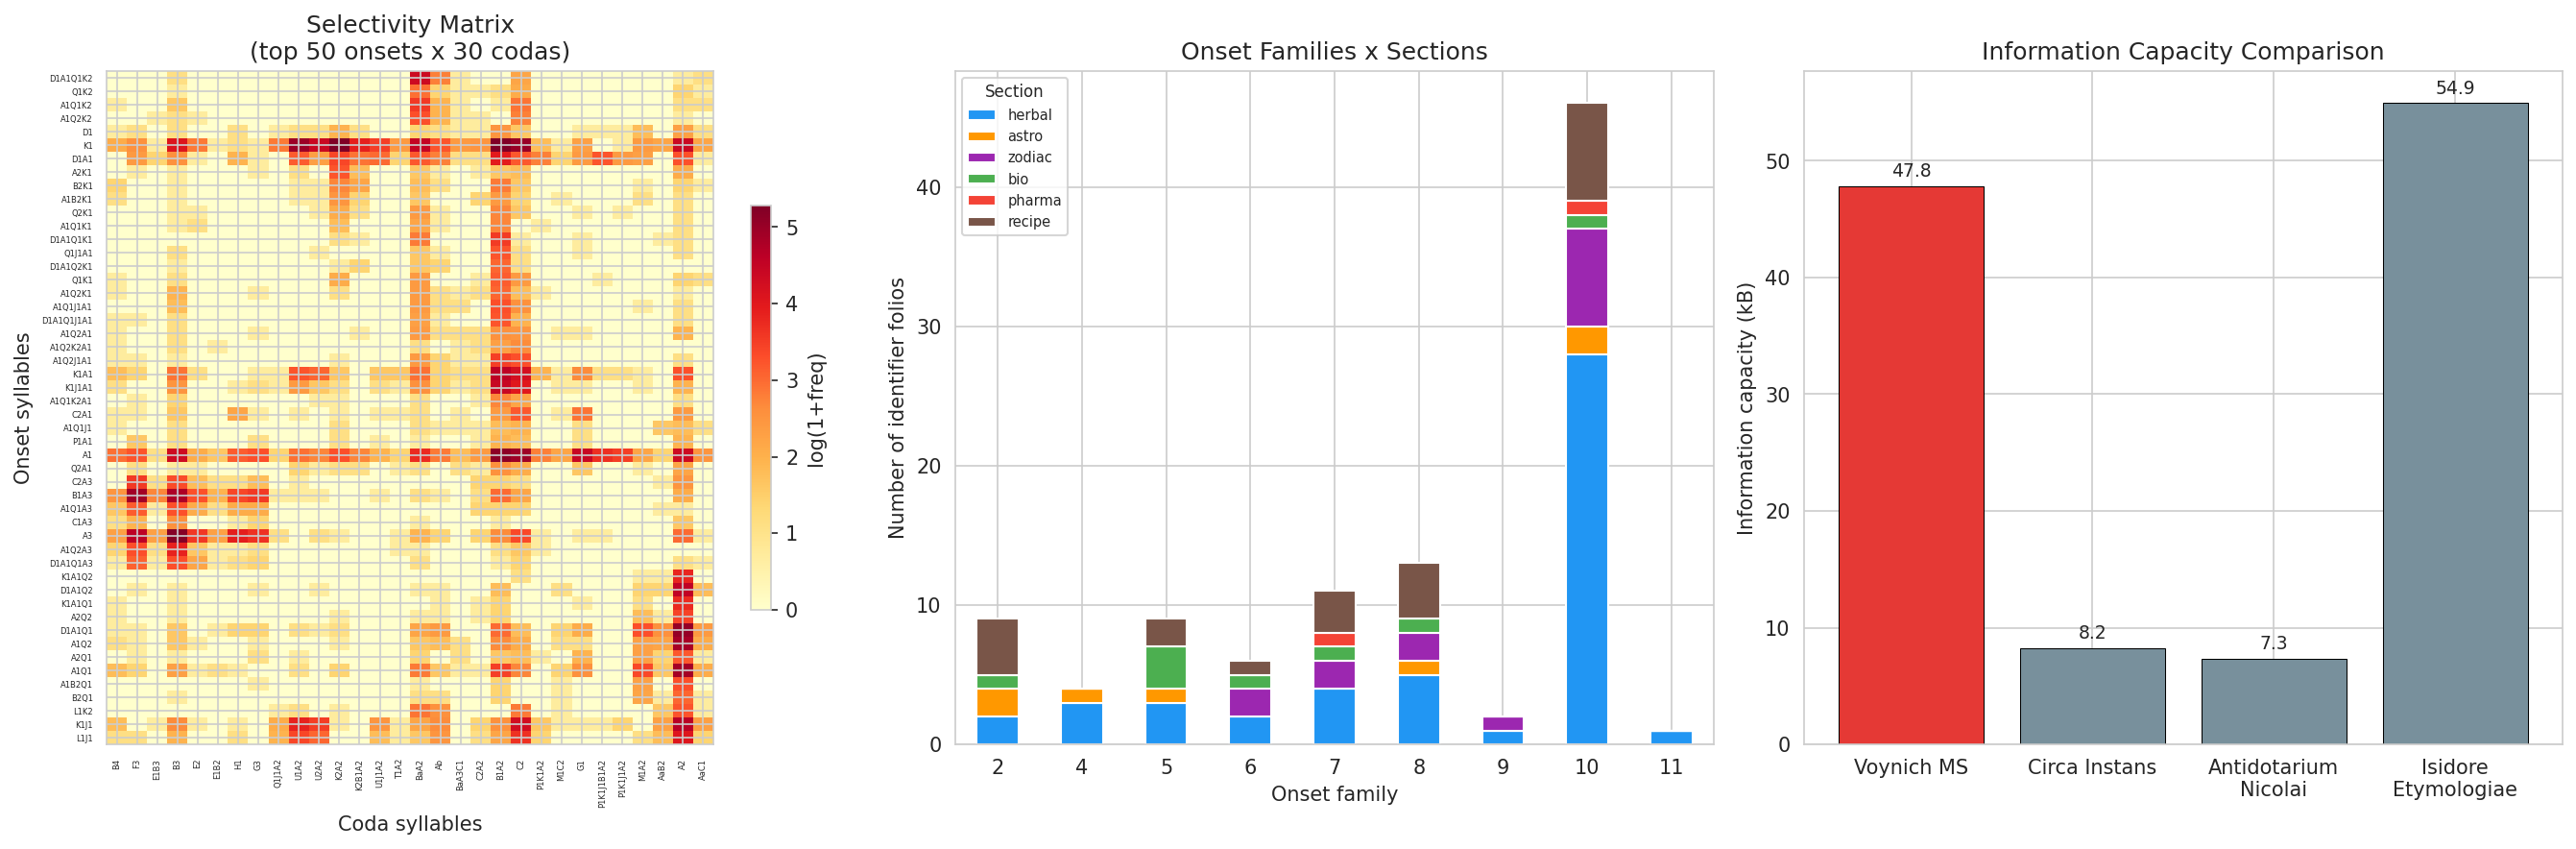
\includegraphics[width=\columnwidth]{code_anatomy.png}
\caption{Code anatomy.  Left: clustered heatmap of the onset $\times$ coda selectivity matrix (88\% sparse), revealing block structure corresponding to onset families.  Centre: onset family sizes and section distribution.  Right: information capacity comparison with historical medieval references.}
\label{fig:anatomy}
\end{figure}

\paragraph{Summary.}
The complete architecture of the Voynich code comprises: 12 onset families (thematic domains), 223 unique entry identifiers, 125 structural elements (markers, headers, modifiers), a three-zone entry structure (identifier $\to$ description $\to$ instructions), and a total information capacity of 48~KB across 226 entries.  Without the author's codebook, we cannot read the content---but we can now describe, quantitatively and in detail, \emph{how} the code is organised, \emph{where} each piece of information sits, and \emph{how much} information the manuscript contains.  The Voynich is not an impenetrable mystery; it is a 48-kilobyte encyclopaedic database whose index has been lost.

\subsection{STA1 Metadata: Illustration Type, Currier Language, and Writing Hand}

The STA1~2.0 transcription embeds rich metadata for each folio: illustration type (\$I: Herbal, Astronomical, Biological, Cosmological, Pharmaceutical, Stars-only, Text-only, Zodiac), Currier language (\$L: A or B---two statistically distinct text populations identified by \citealt{currier1976}), and writing hand (\$H: five identified hands).  Re-running the two-tier analysis with these official classifications---rather than our earlier approximate section assignments by folio number---yields three findings.

\paragraph{Two-tier structure varies by illustration type.}
The Astronomical section has the lowest Tier~1 proportion (27.6\% F) and highest Tier~2 (20.4\% O-C), making it the most ``technical'' section.  The Biological section is the most ``functional'' (61.9\% F).  Crucially, combinatorial utilisation is stable across \emph{all} eight illustration types (range: 4.4\%--6.1\%), confirming that the selectivity constraint ($\sim$93\% of combinations forbidden) is a property of the code system itself, not of any particular section.

\paragraph{Currier's two ``languages'' are two registers of the same code.}
Language~A (\%F~$= 41.8$, \%O-C~$= 14.8$) is more content-heavy, while Language~B (\%F~$= 52.8$, \%O-C~$= 17.0$) is 11 percentage points more functional.  Both maintain the same utilisation ($\sim$6\%) and the same onset/coda ratio ($\sim$1.8).  This suggests that A and B are not two natural languages but two \emph{registers} within a single code: Language~A for detailed item descriptions (lower \%F, more combinatorial content), Language~B for instructions and procedures (higher \%F, more functional markers).

\paragraph{Writing hands correlate with vocabulary communities.}
Chi-squared tests show that the four Louvain vocabulary communities correlate \emph{more strongly} with writing hand ($\chi^2 = 82{,}857$) than with illustration type ($\chi^2 = 79{,}123$) or Currier language ($\chi^2 = 44{,}776$), all at $p \approx 0$.  Community~0 (72~folios) is exclusively Hand~1 / Language~A; Community~2 (52~folios) is Hands~2+3 / Language~B.  Each scribe used a distinct subset of the code vocabulary---not because they wrote in different languages, but because they were responsible for different domains of the encyclopaedia.

\subsection{The Selectivity Matrix and Register Lexicons}

Three final analyses complete the structural picture.

\paragraph{The selectivity matrix.}
The full onset$\times$coda co-occurrence matrix (164 onsets $\times$ 87 codas) has 90\% zero entries---confirming that $\sim$90\% of all possible onset--coda combinations are forbidden.  Hierarchical clustering of the binary matrix reveals 8 onset blocks.  The three most productive onsets (\texttt{K1}, \texttt{A1}, \texttt{D1.A1}) form a ``universal'' block that shares 40 codas---these are the code's workhorses, appearing in every section and combining with nearly half of all available modifiers.  The remaining 7 blocks have 0--8 shared codas each, reflecting domain-specific combinatorial rules.

\paragraph{Register lexicons: A = technical, B = functional.}
Separating Language~A and Language~B vocabularies reveals a stark asymmetry.  A-only word types (2,711) are almost entirely Tier~2 content (\%T2 = 74.6\%, \%F = 4.5\%); B-only types (4,958) are substantially more functional (\%T2 = 59.1\%, \%F = 25.2\%).  Only 1,156 types are shared between registers.  This confirms that the two Currier ``languages'' are two \emph{lexicons} within one code: Language~A encodes item descriptions (technical content), Language~B encodes procedures and instructions (functional scaffolding).  The Herbal section has the highest inter-register overlap (Jaccard = 0.113), while the Biological and Pharmaceutical sections have zero overlap---completely disjoint vocabularies per register.

\paragraph{Isolated folios.}
Sixteen folios form singleton communities in the vocabulary network, sharing no Tier~2 vocabulary with any other folio at Jaccard $> 0.05$.  These isolates are significantly more technical than the rest (\%F = 25.5\% vs.\ 42.0\%), with higher rates of unique (hapax) words.  Many are zodiac folios (f71v, f72r3, f72v1--v2), whose astrological vocabulary is so specialised that it does not overlap with any other section.  The anomalous folio f116v---nearly blank, with only a few lines in what may be a different hand---is among the isolates.

\subsection{Limitations and Future Research}

Several limitations should be noted.

\begin{enumerate}[nosep]
  \item \textbf{Threshold sensitivity.}  The TP-P20 segmentation uses the 20th percentile of transition probabilities as the syllable boundary threshold.  A sweep from P5 to P40 (Fig.~\ref{fig:robustness}) shows that the Tier~1/Tier~2 ratio varies substantially (\%F ranges from 22\% at P40 to 85\% at P5), because more aggressive segmentation creates more multi-syllable (Tier~2) words.  However, the most distinctive property---combinatorial utilisation---is robust: it remains below 12\% at \emph{all} tested thresholds (range: 6.0\%--11.7\%, std = 1.8\%).  The onset$\to$coda transition probability is also robust (CV = 11\%).  The inverted onset/coda ratio ($>$1.0) holds at 7 of 8 thresholds.  Additionally, varying the minimum frequency threshold for syllable classification (freq $\geq$ 3, 5, 10, 20) at fixed P20 leaves \%F unchanged (48.3\% in all cases) and keeps utilisation below 12\%.  P20 represents the mid-point where both tiers are balanced, but the core finding (low utilisation, inverted asymmetry) does not depend on this specific choice.

\begin{figure}[htbp]
\centering
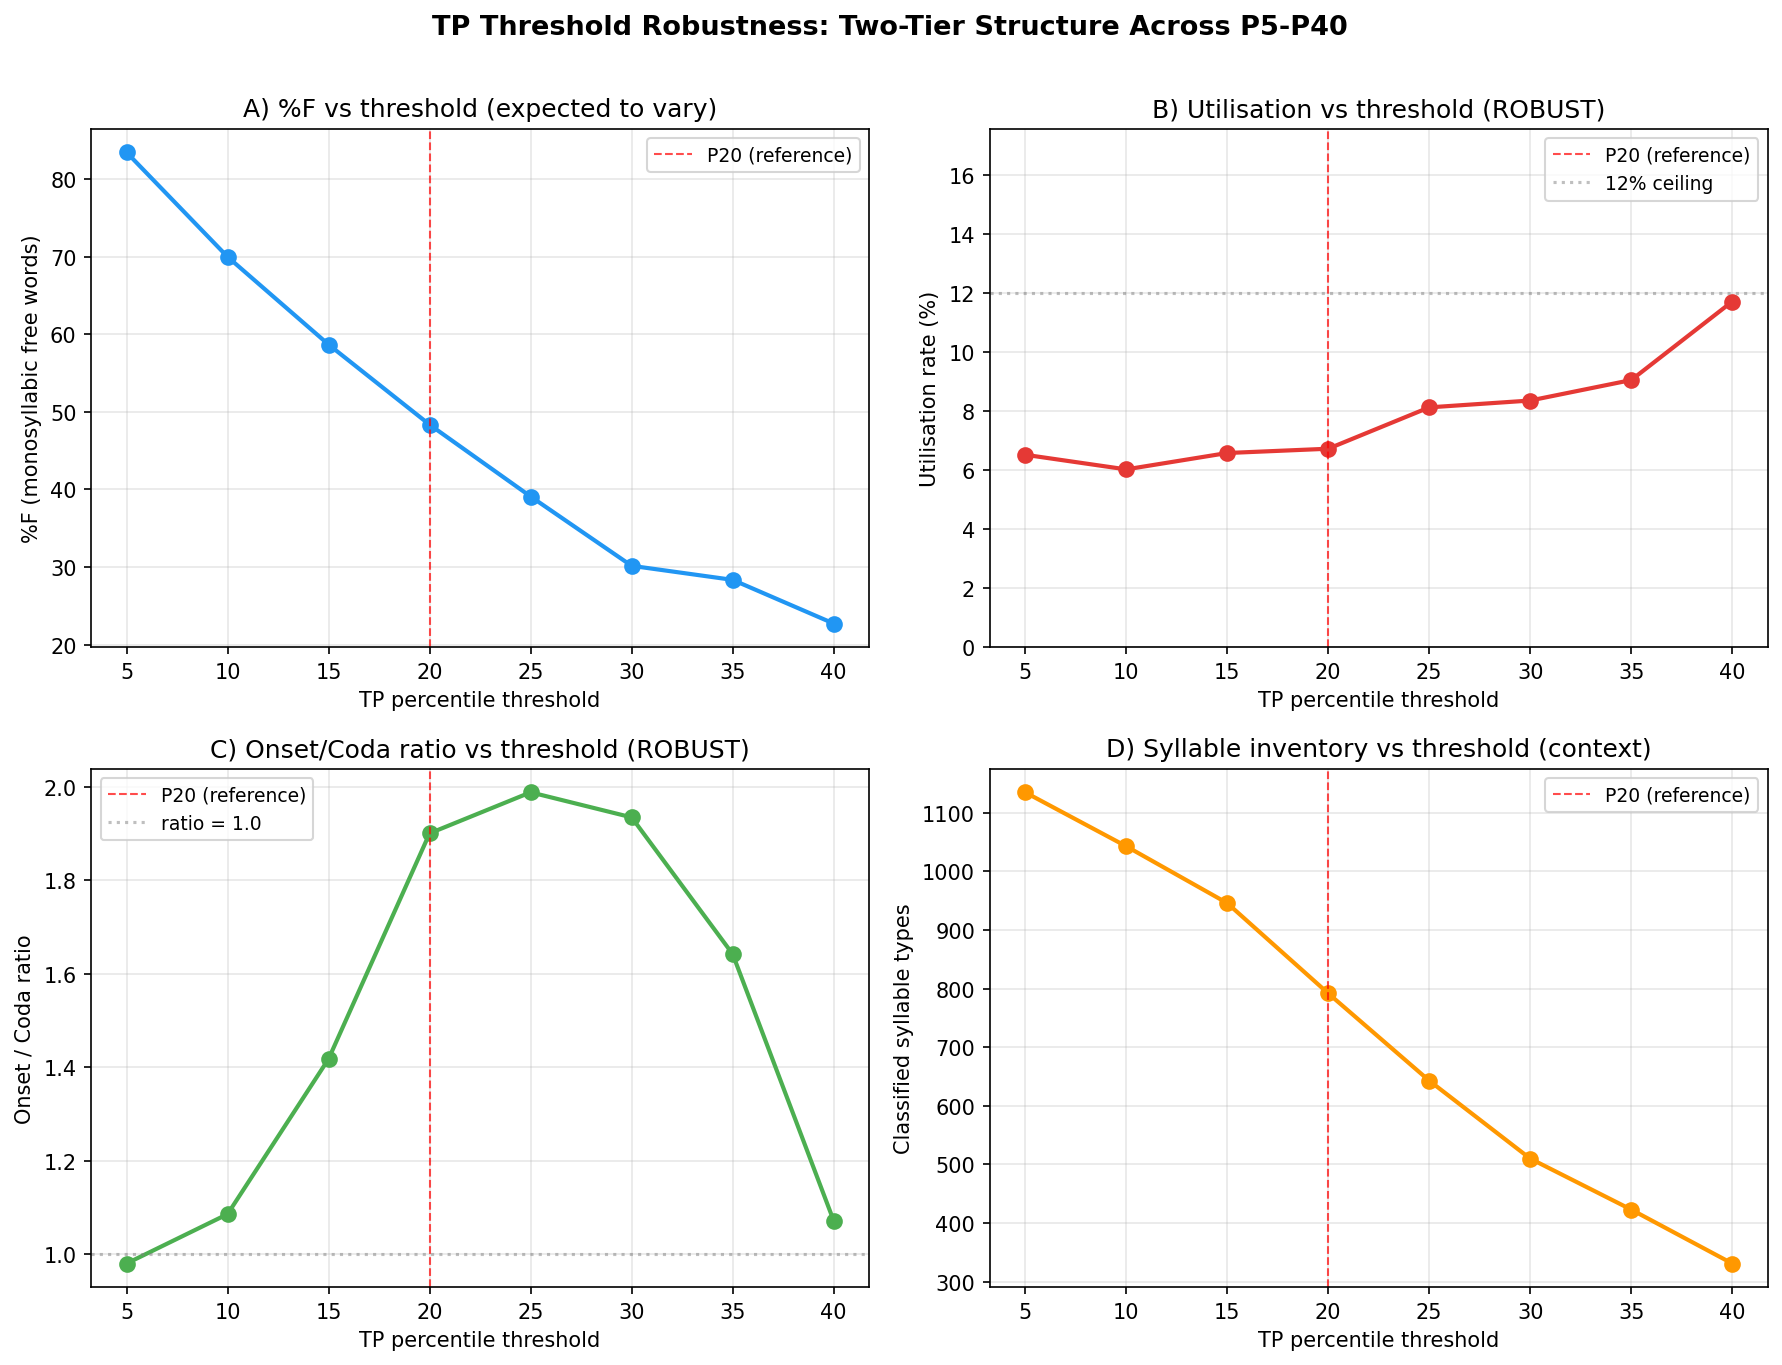
\includegraphics[width=\columnwidth]{tp_threshold_robustness.png}
\caption{Robustness of two-tier metrics across TP segmentation thresholds (P5--P40).  Top left: \%F varies with threshold (expected).  Top right: combinatorial utilisation remains below 12\% at all thresholds (robust).  Bottom left: onset/coda ratio $>$1.0 at 7 of 8 thresholds (robust).  Bottom right: number of classified syllable types.  Dashed line marks the reference P20 threshold.}
\label{fig:robustness}
\end{figure}
  \item \textbf{The two-tier analysis is based on the STA1~2.0 transcription.}  If STA1 over-distinguishes positional glyph variants (creating artificial onset/coda distinctions), the two-tier pattern could be partially artefactual.  However, the EVA transcription (34 types) also shows section differentiation, and the allograph test reduces the STA1 inventory by only 12.7\%, suggesting over-counting is modest.
  \item \textbf{Plant and zodiac identifications are tentative.}  The herbal and zodiac cross-referencing tests rely on subjective identifications from the literature.  More reliable identifications would strengthen (or weaken) the section-level encoding finding.
  \item \textbf{Architecture without semantics.}  The structural decoding identifies \emph{roles} (marker, modifier, category label) but not \emph{meanings}.  A critic may argue that describing the architecture without reading the content is an incomplete result.  We contend that it is nevertheless a significant advance: it reduces the decipherment problem from ``find a mapping from 166 glyphs to an unknown language'' (a space of $>10^{200}$ possibilities) to ``identify $\sim$20 markers, $\sim$21 modifiers, and $\sim$83 section headers in a constrained combinatorial system'' (a space that is finite, enumerable, and potentially solvable with external evidence such as a partial key, a bilingual annotation, or systematic cross-referencing with the manuscript's illustrations).
  \item \textbf{The recipe code simulation is a proof of concept.}  We show that a constrained code \emph{can} reproduce the Voynich utilisation, not that the Voynich \emph{is} such a code.  Alternative systems with different internal logic could produce similar metrics.
  \item \textbf{Within-folio structure.}  If the first word is a functional marker rather than a plant name, the specific content may be encoded at non-initial positions.  Analysing word-position effects within each folio could reveal where content begins after the functional preamble.
\end{enumerate}


% ============================================================
\section{Conclusion}
\label{sec:conclusion}

This paper has reverse-engineered the database schema of the Voynich Manuscript without reading a single word.  Through purely statistical analysis of syllable-position distributions---requiring no assumption about the target language---we have characterised the encoding mechanism at three levels: macro (sections), meso (words), and micro (positions within entries).  Table~\ref{tab:summary} consolidates the quantitative findings.

\begin{table}[htbp]
\caption{Summary of the Voynich code architecture.}
\label{tab:summary}
\centering
\begin{tabular}{ll}
\toprule
\textbf{Property} & \textbf{Value} \\
\midrule
Total entries (folios) & 226 \\
Unique entry identifiers & 223 (98.7\%) \\
Total words & 37,087 \\
Glyph types & 166 \\
Tier~1 (functional) words & 48.3\% \\
Tier~2 (combinatorial) words & 51.7\% \\
Onset--coda utilisation & 6.7\% (90\% forbidden) \\
Onset/coda ratio & 1.95:1 (inverted vs.\ natural languages) \\
Onset blocks (selectivity clusters) & 8 \\
Universal markers & 20 \\
Section-specific headers & 83 \\
Universal modifier codas & 21 \\
Entry zones & 3 (identifier $\to$ description $\to$ instructions) \\
Currier registers & 2 (A = technical 74.6\% T2, 4.5\% F; B = functional 59.1\% T2, 25.2\% F) \\
Vocabulary communities & 4 (correlate with scribe + register) \\
Isolated folios & 16 (mostly zodiac, ultra-specialised) \\
Information capacity & 48~KB (226 entries $\times$ 1,730 bits) \\
\bottomrule
\end{tabular}
\end{table}

Ten principal findings emerge:

\begin{enumerate}[nosep]
  \item The text has a \textbf{two-tier structure}: 48\% self-contained functional words (Tier~1, Zipf $\alpha = 1.16$) and 52\% combinatorial content words (Tier~2, Zipf $\alpha = 0.64$), with distinct statistical signatures.
  \item Only \textbf{6.7\% of onset--coda combinations} are attested---reproducible only by a constrained code with $\sim$90\% of combinations forbidden.  No natural language or unconstrained code matches this selectivity.
  \item Each entry begins with a \textbf{unique identifier} (98.7\% uniqueness), followed by a description zone and an instruction zone---the structure of a catalogue entry.
  \item \textbf{Onset syllables encode section-level categories} (Cram\'er's $V = 0.088$, $p < 10^{-94}$) while \textbf{codas encode cross-cutting modifiers} ($V = 0.067$)---but neither encodes individual items within a section.
  \item The \textbf{selectivity matrix} reveals 8 onset blocks organised by frequency tier (3 universal onsets sharing 40 codas, down to 57 rare onsets with no shared codas), not by thematic domain.
  \item Currier's two ``languages'' (A and B) are \textbf{two registers} of the same code: A-exclusive vocabulary is 74.6\% Tier~2 content with only 4.5\% functional words; B-exclusive vocabulary is 59.1\% Tier~2 with 25.2\% functional.  Both registers maintain the same utilisation ($\sim$6\%) and onset/coda ratio ($\sim$1.8).
  \item \textbf{Vocabulary communities correlate with writing hand} ($\chi^2 = 82{,}857$) more than with illustration type ($\chi^2 = 79{,}123$): each scribe was responsible for a different domain of the encyclopaedia.
  \item The system's closest parallels are \textbf{Esperanto} (regular morphology, distance 1.03) and \textbf{Lingua Ignota} (inverted onset/coda ratio, distance 1.30)---both rule-based constructed systems.
  \item The total \textbf{information capacity} is 48~KB---consistent with a medieval multi-domain technical reference such as the \textit{Circa Instans} or the \textit{Antidotarium Nicolai}.
  \item All structural properties are \textbf{robust} to the segmentation threshold (utilisation $< 12$\% across P5--P40) and to minimum frequency thresholds.
\end{enumerate}

These findings shift the Voynich question from ``what language is encoded?'' to ``what kind of system produced this text?''  The answer, supported by every analysis in this paper, is: \textbf{an encyclopaedic code}---a personal technical reference system in which the encoding mechanism \emph{is} the content, each scribe contributed a domain, and the author's codebook is the missing key.

Any future proposal for the Voynich Manuscript must account for the two-tier combinatorial structure, the 90\% selectivity, the three-zone entry format, and the register/scribe partitioning documented here.  Without the codebook, we cannot read the content---but we now know, quantitatively and in detail, \emph{how} the code is organised, \emph{where} each piece of information sits, and \emph{how much} information the manuscript contains.  The Voynich Manuscript is not an impenetrable mystery; it is a 48-kilobyte encyclopaedic database whose index has been lost.


% ============================================================
% END MATTER
% ============================================================

\section*{Data Availability}

The Voynich corpus (STA1~2.0 transcription) is publicly available at \url{https://www.voynich.nu/transcr.html}.  All analysis code (notebooks 36--48) and results are available at \url{https://github.com/cesarjz/Voynich}.

\section*{AI Disclosure Statement}

This manuscript was prepared with the assistance of Claude (Anthropic, version Claude Opus 4).  The author used the tool to assist with code development for the computational notebooks, to help draft and edit the manuscript text, and to generate structured outputs from experimental results.  All content generated by the tool was checked and approved by the author.

\section*{Funding}

This research received no specific grant from any funding agency in the public, commercial, or not-for-profit sectors.

\section*{Acknowledgements}

The Voynich Manuscript transcription data are from the STA1~2.0 corpus by Ren\'e Zandbergen.  The Ge'ez corpus is from the TraCES project (University of Hamburg).  Hebrew and Aramaic texts were obtained from the Sefaria digital library.  The author's interest in the manuscript was deepened by a visit to the Silo\'e editorial workshop in Burgos, Spain (\url{https://siloe.es/facsimiles/manuscrito-voynich/}), whose facsimile edition reproduces the original with remarkable fidelity using period techniques.


\bibliographystyle{abbrvnat}
\bibliography{twotier_paper}

\end{document}
